\documentclass[4pt,margin=0.9in,innermargin=-1.50in,blockverticalspace=-0.001in]{tikzposter}
\geometry{paperwidth=36in,paperheight=48in}
\usepackage[utf8]{inputenc}
\usepackage{amsmath,amsfonts,amsthm,amssymb}
\usepackage{array,colortbl}
\usepackage{mathrsfs}
\usepackage{graphicx}
\usepackage{adjustbox}
\usepackage{enumitem}
\usepackage[backend=biber,style=numeric]{biblatex}
\usepackage{emory-theme}
\usepackage{tikz}
\usepackage[utf8]{inputenc}
\usepackage{longtable}
\usetikzlibrary{calc,chains,backgrounds,positioning,matrix,decorations.markings,arrows,arrows.meta}
\usepackage{pdfpages}
\usepackage{pgfplots}
\pgfplotsset{compat=1.7}
\usepackage{listings}
\usepackage{xcolor}
\usepackage{listings}
\usepackage{multirow}

%% For code listings
\definecolor{codegreen}{rgb}{0,0.6,0}
\definecolor{codegray}{rgb}{0.5,0.5,0.5}
\definecolor{codepurple}{rgb}{0.58,0,0.82}
\definecolor{backcolour}{rgb}{0.95,0.95,0.92}
\lstdefinestyle{mystyle}{
  backgroundcolor=\color{backcolour},   
  commentstyle=\color{codegreen},
  keywordstyle=\color{magenta},
  numberstyle=\tiny\color{codegray},
  stringstyle=\color{codepurple},
  basicstyle=\ttfamily\footnotesize,
  breakatwhitespace=false,         
  breaklines=true,                 
  captionpos=b,                    
  keepspaces=true,                 
  numbers=left,                    
  numbersep=5pt,                  
  showspaces=false,                
  showstringspaces=false,
  showtabs=false,                  
  tabsize=2
}

\lstset{
  escapeinside={{*@}{@*}}
}

\usepackage{mwe} % for placeholder images


% Custom Macros
\newcommand{\MiddFS}[2]{#1{M}#2{iddFS }#1{i}#2{s'nt mi}#1{d}#2{\quad \quad}#1{d}#2{\quad \quad}#1{F}#2{ile\quad}#1{S}} % #1 large; #2 small
\newcommand{\middfs}{\texttt{middfs}}
\newcommand{\rc}{\rowcolor}

% set theme parameters
\tikzposterlatexaffectionproofoff
\usetheme{EmoryTheme}
\usecolorstyle{EmoryStyle}

\title{\texttt{ZC} -- an (e)Z80 Compiler}
\author{\vspace{1cm} Nicholas Mosier '20 \\ \vspace{1cm} \small \texttt{https://github.com/nmosier/zc.git}}
\titlegraphic{\includegraphics[width=0.2\textwidth]{mdl_master_left_blue.png}}

% begin document
\begin{document}
\maketitle

\centering

\begin{columns}
  \column{0.5}
  \block{Introduction \& Motivation}{
    The Zilog Z80, a CISC 8-bit microprocessor that used to be ubiquitious in personal computing and arcade gaming in the 1970-80's, is still used to this day in Texas Instrument's TI-83/84+ graphing calculators. More recently, the eZ80 processor, introduced in the early 2000's, features a minor, backwards-compatible update to the original Z80 ISA, and is used in the TI's higher-end calculators, e.g. the TI-84+ CE. TI calculator programmers (including me), 

    \begin{itemize}
    \item No C compilers target both the Z80 and eZ80.
    \item Large code size output of existing C compilers targeting the eZ80.
    \end{itemize}

    To address this need, we introduce ZC, an optimizing C compiler for the eZ80 (and, eventually, the Z80 as well).

  }

  \block{Compiler Anatomy}{
    ZC accepts a C source file as input and produces (e)Z80 assembly as output.
    The ZC compiler frontend parses the input file into an
    {\it abstract syntax tree} (AST) and annotates it with type information,
    while the ZC backend translates the abstract syntax tree into a control flow
    graph, performs optimization, and outputs an (e)Z80 assembly instruction stream.

    \begin{minipage}{0.5\linewidth}
    \innerblock{Frontend}{
      {\bf Lexer and parser:}
      The lexer and parser, written for the {\tt flex} and {\tt bison} tools,
      implement the C grammar and define the rules for constructing an AST
      representing the input program.

      {\bf Semantic Analysis:}
      The ZC compiler infers the types of expressions in the AST,
      resolves user-defined types such as {\tt struct}s and {\tt typedef}s,
      and checks semantic validity of the program.
    }
    \end{minipage}
    \begin{minipage}{0.5\linewidth}
    \innerblock{Backend}{
      {\bf Code Generation:}
      For each function definition, ZC generates a control flow diagram of
      basic blocks containing symbolic (e)Z80 instructions and determines
      an activation record layout.

      {\bf Register allocation: }
      ZC traverses the control flow graph and assigns registers or memory locations
      to all variables created during code generation.
    }
    \end{minipage}

    \tikzset{
      brace/.style={
        decoration={brace,amplitude=0.5cm},
        decorate
      }
    }
    \tikzstyle{ar} = [arrows={-Triangle[scale=2]}]
    
    \begin{tikzfigure}
      \begin{tikzpicture}[
        start chain,
        node distance=1cm,
        zc/.style={draw,on chain,align=center,join=by ar},
        zcl/.style={node distance=5cm},
        zcb/.style={brace,decoration={raise=4ex}},
        ]

        \node[zc] (src) {C \\ source};
        \node[zc] (lexer) {Lexer \\ ({\tt flex})};
        \node[zc] (parser) {Parser \\ ({\tt bison})};
        \node[zc] (semant) {Semantic \\ Analysis};
        \node[zc] (astopt) {AST \\ Optim.};
        \node[zc] {Code \\ Gen.};
        \node[zc] (ralloc) {Register \\ Alloc.};
        \node[zc] (asmopt) {Asm \\ Optim.};
        \node[zc] (asm) {Asm};

        \node[zcl] (in) [above of=src] {Input};
        \node[zcl] (out) [above of=asm] {Output};

        \node[zcl] (frontend) [above of=parser] {Frontend};
        \node[zcl] (backend) [above of=ralloc] {Backend};

        \draw[zcb] (lexer.north west) -- (semant.north east);
        \draw[zcb] (astopt.north west) -- (asmopt.north east);
        
      \end{tikzpicture}
      
    \end{tikzfigure}

  }

  \block{Register Allocation} {

    % Stack Machine vs. Register Allocation
    \begin{minipage}{0.5\linewidth}
      \innerblock{Stack Machine}{
        When evaluating expressions, a stack-machine compiler pushes intermediate
        values (e.g. the left-hand side of an addition)
        onto the stack and pops them off when it is ready to be combined with another
        intermediate value (e.g. added to the right-hand side of an addition).
        A stack machine is easy to implement; the first version of ZC's code generator
        was a stack machine.
      }
    \end{minipage}
    \begin{minipage}{0.5\linewidth}
      \innerblock{Register Allocation}{
        A compiler with a register allocator moves intermediate values into registers
        rather than pushing them onto the stack.
        However, there are often more intermediate values
        than there are physical registers.
        For example, the (e)Z80 has {\bf 7 byte registers}
        but only {\bf 3 allocatable multibyte registers}.
        When intermediate values exceed physical registers in number,
        those values must be \textit{spilled} into memory.
      }
    \end{minipage}

    \begin{minipage}{0.5\linewidth}
    \innerblock{(e)Z80 Restrictions}{
      The (e)Z80's instruction set is accumulator-based:
      most operations aside from moves require the destination and first operand
      to be the byte register {\tt a} or the multibyte register {\tt hl}.
      Traditional register allocation does not account for this bias,
      so our ZC compiler implements a specialized register allocation algorithm
      that accounts for some operands being fixed registers and others
      being unbound variables.
      
    }
    \end{minipage}
    \begin{minipage}{0.5\linewidth}
    \innerblock{Frame vs. Stack Spilling in ZC}{
      Most compilers spill intermediate values into the callee's frame
      (i.e. activation record), also where local variables are stored -- we call this
      {\it frame spilling}.
      On the (e)Z80, however, accessing memory through the frame pointer register
      {\tt ix} is costly;
      it is much more efficient to push/pop intermediate values directly to/from the
      stack -- we call this {\it stack spilling}.
      Stack spilling is cheap but restrictive; frame spilling is costly but versatile.
      If a value cannot be assigned a register, ZC tries to spill onto the stack,
      resorting to frame-spilling if it fails.
    }
    \end{minipage}

    \begin{tikzfigure}
    {\tt
      \begin{tabular}{>{\bf}ll|>{\bf}ll|>{\bf}ll}
        \multicolumn{2}{c|}{\bf Stack Machine}
        & \multicolumn{4}{c}{\bf Register Allocation} \\
        & & \multicolumn{2}{c}{\rm Before} & \multicolumn{2}{c}{\rm After}
        \\\hline
        ld & a,(ix+7) & ld & {\it vb4} ,(ix+7) & ld & a,(ix+7) \\
        push & af & & & & \\
        ld & a,97 & ld & {\it vb5},97 & ld & l,97 \\
        pop & bc & ld & a,{\it vb4} & ld & a,a \\
        cp & a,b & cp & a,{\it vb5} & cp & a,l \\
      \end{tabular}
    }
    \end{tikzfigure}

    
  }
    
  \block{Optimizations Overview}{

    \begin{itemize}
    \item Peephole optimization
    \item Register allocation
    \item Constant evaluation
    \item Reducing boolean conversions
    \item Transitions minimization
    \item Direct calls
    \end{itemize}
    
  }
  
  \column{0.5}

  
  \block{Results}{
    \begin{tikzfigure}
      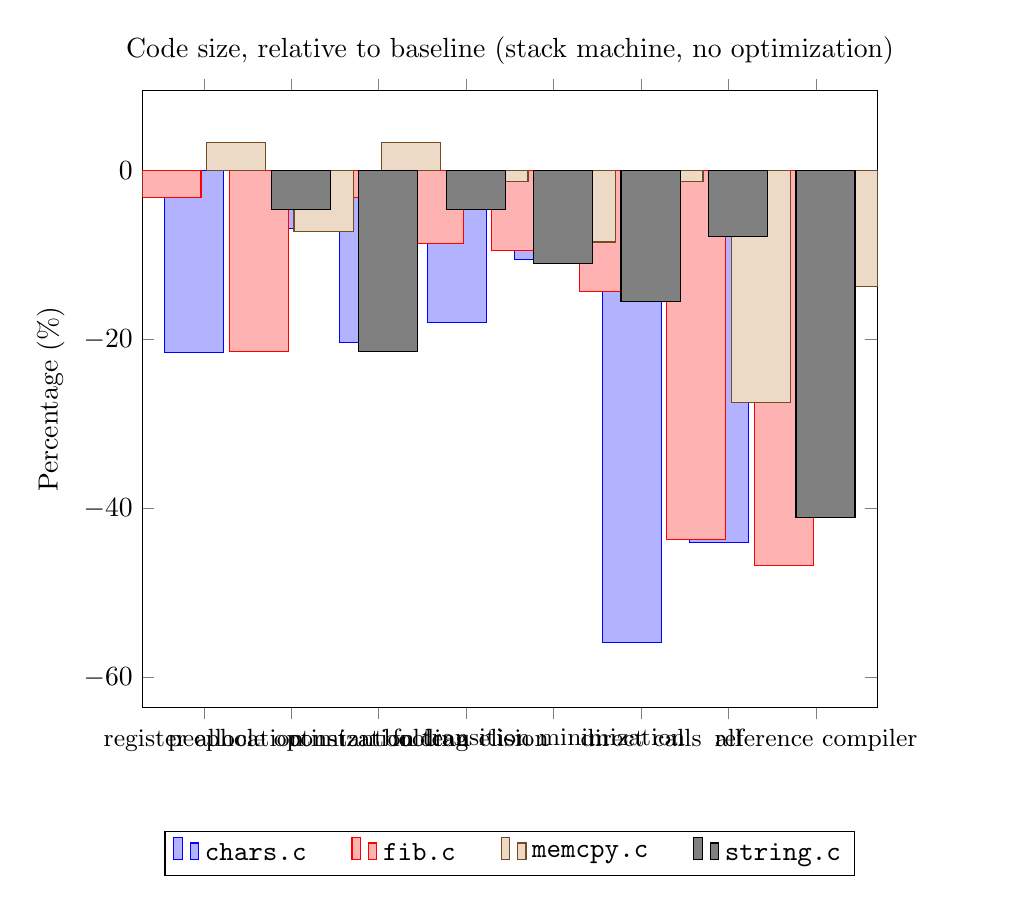
\begin{tikzpicture}
        \begin{axis}[
          width=0.9\linewidth,
          ybar,
          symbolic x coords={register allocation, peephole optimization, constant folding, boolean elision, transition minimization, direct calls, all, reference compiler},
          enlarge x limits=true,
          xtick=data,
          ytick={0,20,40,60,80,-20,-40,-60},
          ylabel={Percentage (\%)},
          legend style={
            at={(0.5, -0.2)},
            anchor=north,
            legend columns=-1,
            /tikz/every even column/.append style={column sep=0.5cm}
          },
          x tick label style={font=\small, text width=4cm, align=center},
          bar width=0.75cm,
          title={Code size, relative to baseline (stack machine, no optimization)},
          ]

          % chars.c
          \addplot coordinates {
            (register allocation,-4.9)
            (peephole optimization,-21.6)
            (constant folding,-6.9)
            (boolean elision,-20.4)
            (transition minimization,-18.0)
            (direct calls,-10.6)
            (all,-55.9)
            (reference compiler,-44.1)
          };
          

          % fib.c
          \addplot coordinates {
            (register allocation,-3.2)
            (peephole optimization,-21.4)
            (constant folding,-3.2)
            (boolean elision,-8.7)
            (transition minimization,-9.5)
            (direct calls,-14.3)
            (all,-43.7)
            (reference compiler,-46.8)
          };

          % memcpy.c
          \addplot coordinates {
            (register allocation,3.3)
            (peephole optimization,-7.2)
            (constant folding,3.3)
            (boolean elision,-1.3)
            (transition minimization,-8.5)
            (direct calls,-1.3)
            (all,-27.5)
            (reference compiler,-13.8)
          };

          % string.c
          \addplot coordinates {
            (register allocation,-4.6)
            (peephole optimization,-21.5)
            (constant folding,-4.6)
            (boolean elision,-11)
            (transition minimization,-15.5)
            (direct calls,-7.8)
            (all,-41.1)
            (reference compiler,-57.5)
          };

          \legend{\texttt{chars.c}, \texttt{fib.c}, \texttt{memcpy.c},
            \texttt{string.c}}

        \end{axis}
      \end{tikzpicture}
    \end{tikzfigure}

    \innerblock{}{
    \begin{tikzfigure}
      % \begin{table}
        \begin{tabular}{|c|c|c|c|c|}\hline
          & {\tt chars.c} & {\tt fib.c} & {\tt memcpy.c} & {\tt string.c} \\\hline
          {\bf stack machine} & {\bf 245} & {\bf 126} & {\bf 305} & {\bf 219} \\\hline
          register allocation & 233 & 122 & 313 & 208 \\\hline
          peephole optimization & 192 & 99 & 283 & 173 \\\hline
          constant folding & 228 & 122 & 315 & 208 \\\hline
          boolean elision & 195 & 115 & 301 & 194 \\\hline
          transition minimization & 201 & 114 & 279 & 176 \\\hline
          direct calls & 219 & 108 & 301 & 201 \\\hline
          {\bf all} & {\bf 108} & {\bf 71} & {\bf 221} & {\bf 122} \\\hline
          {\it reference compiler} & {\it 137} & {\it 67} & {\it 263} & {\it 93} \\\hline
        \end{tabular}
      % \end{table}
    \end{tikzfigure}
    }
}
\block{Optimization Examples}{
  {\tt
    \begin{tabular}{>{\bf}ll}
      \rowcolor{gray} or   & a,a   \\
      \rowcolor{gray} sbc  & hl,hl \\
      \rowcolor{gray} ld   & l,a   \\
      \rowcolor{red} push & hl    \\
      \rowcolor{red} pop  & hl \\
      \rowcolor{gray} jp & label0 \\
    \end{tabular}
  }

  \bigskip
  
  {\tt
    \begin{tabular}{>{\bf}ll}
      \rowcolor{red} lea & ix,ix+0 \\
      \rowcolor{red} ld & sp,ix \\
      \rowcolor{gray} pop & ix \\
      \rowcolor{gray} ret \\
    \end{tabular}
  }

  \bigskip

  {\tt
    \begin{tabular}{>{\bf}ll}
      \rc{gray} ld & l,'A' \\
      \rc{gray} cp & a,l \\
      \rc{red} sbc & a,a \\
      \rc{red} inc & a \\
      \rc{red} or & a,a \\
      \rc{red} jp & nz,label0 \\ \rc{green} jp & nc,label0 \\
      \rc{red} jp & z,label1 \\ \rc{green} jp & c,label1 \\
    \end{tabular}
  }
}

  \block{Future Work}{
    Blah, blah, blah.
  }
  

\end{columns}
\end{document}
